\section{Radial Symmetry Kernel Asumnption}
% --- SLIDE 4.5: THE SPHERICAL ESTIMATOR (THE BRIDGE) ---
\begin{frame}{Alternative Simplification: Radial Symmetry}
    \small
    Instead of multiplying univariate kernels, what if we use a single \textbf{Radially Symmetric} kernel $K$ for the whole $p$-dimensional space?

    \vspace{0.5em}

    % 1. THE FORMULA (Equation 10.42)
    \begin{block}{The Spherical Estimator (Eq. 10.42)}
        We use a \textbf{single scalar bandwidth} $h$ for all dimensions:
        \begin{equation}
            \hat{f}(\vect{x}) = \frac{1}{n h^p} \sum_{i=1}^{n} K \left( \frac{\vect{x} - \vect{X}_i}{h} \right)
        \end{equation}
        {\footnotesize \textit{(Where $K$ depends only on the distance $||\vect{x} - \vect{X}_i||$, e.g., Multivariate Epanechnikov)}}
    \end{block}

    \vspace{0.5em}

    % 2. THE GEOMETRY & LIMITATION
    \begin{columns}[c]
        % Left: Characteristics
        \begin{column}{0.55\textwidth}
            \begin{itemize}
                \setlength\itemsep{0.8em}
                \item<2-> \textbf{Geometry:} The kernel shape is a perfect \textbf{Hyper-Sphere} (Ball).
                \item<3-> \textbf{Simplicity:} Only 1 parameter ($h$) to tune!
                \item<4-> \textbf{\textcolor{red}{The Catch:}} It assumes data spreads \textbf{equally} in all directions.
            \end{itemize}
        \end{column}

        % Right: Visual Mismatch
        \begin{column}{0.45\textwidth}
            \centering
            \onslide<4->{
                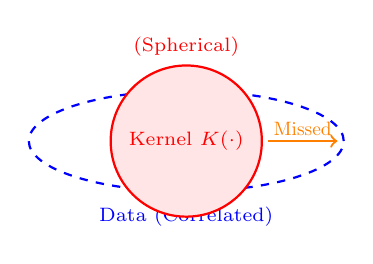
\begin{tikzpicture}[scale=0.8]
                    % Data distribution (Ellipse)
                    \draw[thick, dashed, blue] (0,0) ellipse (2.5cm and 0.8cm);
                    \node[blue] at (0, -1.2) {\scriptsize Data (Correlated)};

                    % Kernel (Circle) - Trying to fit
                    \draw[thick, red, fill=red!10] (0,0) circle (1.2cm);
                    \node[red] at (0, 0) {\scriptsize Kernel $K(\cdot)$};
                    \node[red] at (0, 1.5) {\scriptsize (Spherical)};

                    % Arrows indicating mismatch
                    \draw[->, orange, thick] (1.3,0) -- (2.4,0);
                    \node[orange, scale=0.7] at (1.85, 0.2) {Missed};
                \end{tikzpicture}

                \vspace{0.5em}
                \footnotesize \textcolor{red}{Problem:} A sphere fits poorly inside a long ellipse.
            }
        \end{column}
    \end{columns}

    % 3. TRANSITION TO WHITENING
    \vspace{1em}
    \centering
    \onslide<5->{
        \textbf{Idea:} \textit{If the Kernel can't stretch to fit the Data, why don't we \textbf{shrink the Data} to fit the Kernel?} \\
        \Large $\Downarrow$ \\
        \normalsize \textbf{Next Step: Whitening}
    }
\end{frame}